\documentclass[11pt, a4paper]{article}

% --- 패키지 로드 ---
\usepackage{kotex} % 한글 지원
\usepackage[utf8]{inputenc}
\usepackage{amsmath} % 수식 지원
\usepackage{amsfonts}
\usepackage{amssymb}
\usepackage{geometry} % 여백 설정
\usepackage{booktabs} % 표 디자인
\usepackage{graphicx} % 이미지 삽입
\usepackage{hyperref} % 하이퍼링크
\usepackage{enumitem} % 리스트 설정
\usepackage{float}

% --- 용지 여백 설정 ---
\geometry{top=2.5cm, bottom=2.5cm, left=2cm, right=2cm}

% --- 제목 및 저자 정보 ---
\title{\textbf{시계열 분석을 활용한 서울시 공공자전거(따릉이) \\ 수요 예측 연구 계획서}}
\author{시계열 분석 및 실습 001 \\ [1ex] 2조: 강채림, 박준영, 박현수, 송민석}
\date{\today}

\begin{document}
	
	\maketitle
	
	\section{연구의 배경 및 목적}
	\subsection{연구 배경}
	서울시 공공자전거 ‘따릉이’는 도시 교통의 유연성을 높이는 핵심 모빌리티로 자리 잡았으나, 특정 시간대와 지역에 따른 수요-공급 불균형 문제는 여전히 운영상의 고질적인 난제로 남아 있다. 특히 출퇴근 및 주말 여가 시간대의 폭발적인 수요는 거치대 부족 혹은 자전거 고갈 현상을 야기한다. 시계열 분석을 통한 정밀한 수요 예측은 이러한 운영 비효율성을 타개하기 위한 필수적인 선결 과제이다.
	
	\subsection{연구 목적}
	본 연구는 시공간적 데이터에 기반한 수요 예측 모델을 구축하여, 자전거 재배치의 우선순위와 최적 경로를 도출하고 운영 효율화를 위한 데이터 기반의 정책적 근거를 마련하는 데 목적이 있다.
	
	\section{데이터 수집 및 분석 대상}
	\begin{itemize}
		\item \textbf{데이터 소스:} ‘서울 열린데이터 광장’ 공공자전거 대여 이력 정보 및 대여소 마스터 정보
		\item \textbf{분석 범위:} 최근 5년간(2021.01-2025.12)의 시계열 데이터를 활용하며, 단기적 변동성과 주기성을 동시에 포착하기 위해 \textbf{1시간 단위} 집계 데이터를 분석 단위로 설정한다. 대상 대여소는 서울시 전체 대여소 중 분석 대상인 서울대학교 인근 23개 대여소 ID를 추출히여 사용한다.
		\item \textbf{데이터 전처리 계획:}
		\begin{itemize}
			\item \textbf{재구조화:} 개별 대여 이력을 시간별 대여 횟수로 재집계(Resampling)하여 모델링에 최적화된 형태로 변환한다. 또한 주말과 평일의 다른 추세 형태를 감안하여 평일과 주말 데이터를 분리한다.
		\end{itemize}
	\end{itemize}
	
	\section{탐색적 데이터 분석(EDA) 결과 요약}
	따릉이 수요는 시간별, 월별 단위로 매우 뚜렷한 주기성과 기상 요인에 따른 변동성을 보인다.
	
	\subsection{시간대별 및 월별 패턴 분석}
	\begin{itemize}
		\item \textbf{시간대별 패턴:} 평일은 전형적인 패턴(08시, 18시 피크)을 보이나, 주말은 오전 피크 없이 17~18시 사이에 강한 피크(약 4,500건)가 발생한다. 이는 주말 오후 수요가 평일 오전 피크를 상회할 정도로 집중됨을 의미한다.
        \item \textbf{월별 추이:} 겨울철 급감 후 봄~가을 사이 수요가 유지되나, \textbf{7월 장마철}에는 일시적으로 수요가 하락하는 'V자형' 패턴이 관찰된다. 이러한 비정상성 요소를 모델에 반영한다.
	\end{itemize}
    \begin{figure}[H]
    \centering
    % 왼쪽 그림
    \begin{minipage}{0.48\textwidth}
        \centering
        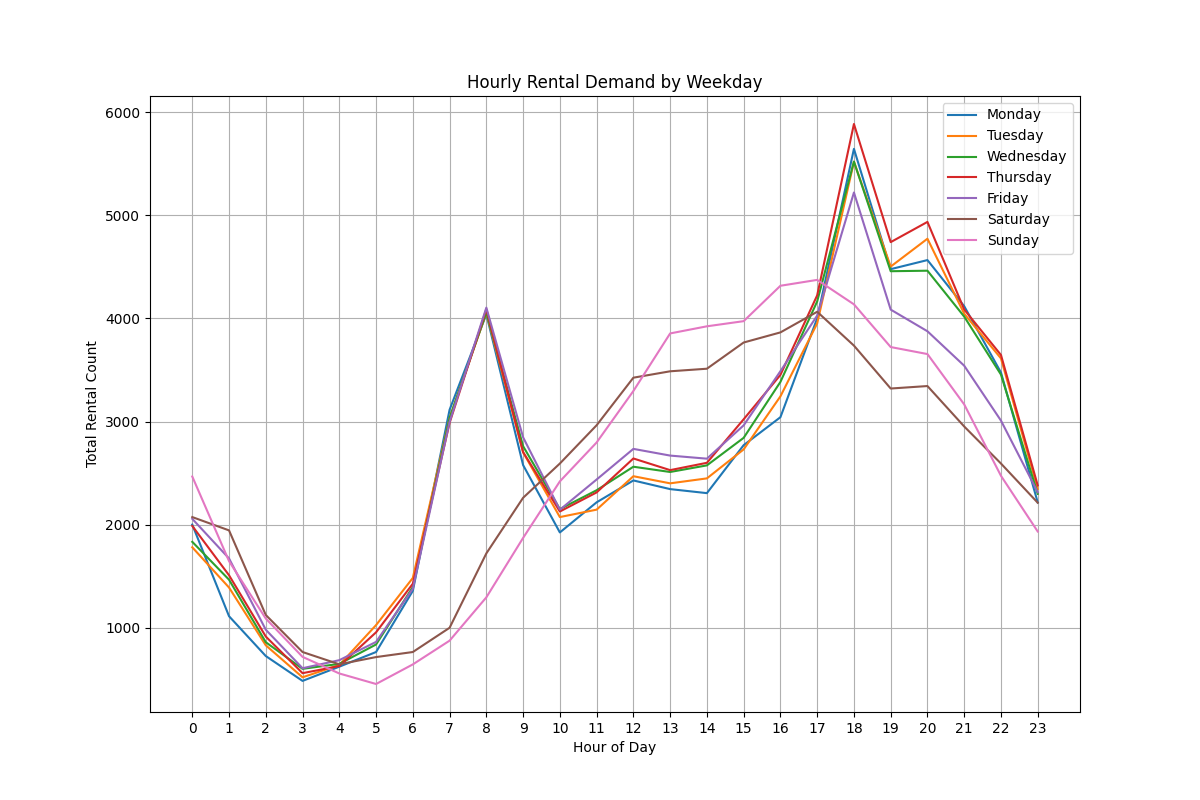
\includegraphics[width=\textwidth]{hourly_demand.png}
        \caption{시간대별 패턴}
    \end{minipage}
    \hfill % 두 그림 사이를 벌려줌
    % 오른쪽 그림
    \begin{minipage}{0.48\textwidth}
        \centering
        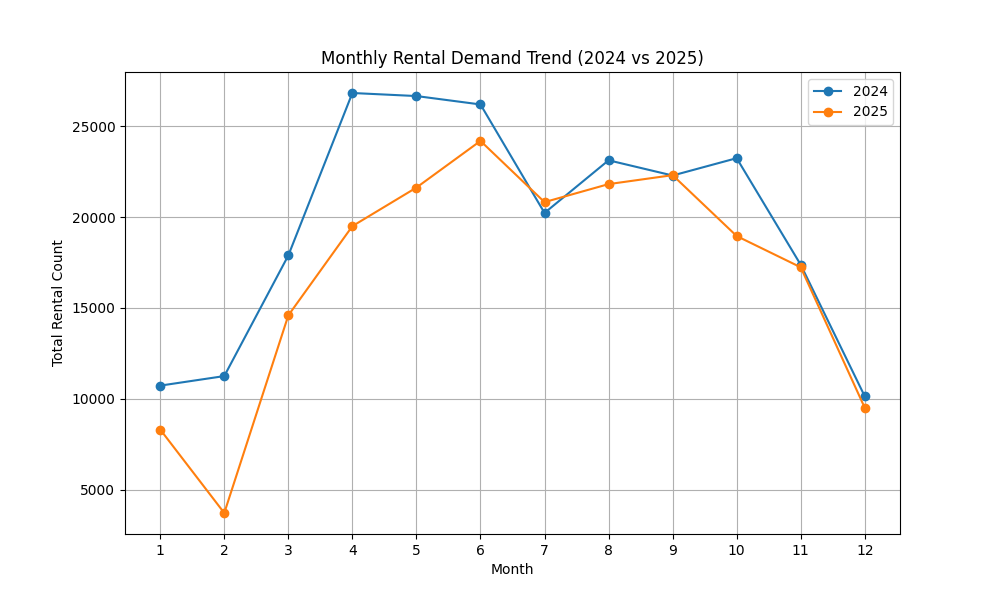
\includegraphics[width=\textwidth]{monthly_demand.png}
        \caption{월별 추이}
    \end{minipage}
\end{figure}
	
	\section{연구 방법론 및 모델링}
	\subsection{수요 예측 모델: SARIMA 및 다중 계절성 반영}
따릉이 대여 수요 데이터는 24시간 단위의 일일 주기와 $24 \times 365$시간 단위의 연간 주기가 복합적으로 작용하는 강력한 다중 계절성을 띤다. 본 연구에서는 이를 효과적으로 모델링하기 위해 다음과 같은 단계적 접근 방식을 취한다.

첫째, 데이터의 평일과 주말의 다른 추세를 반영하기 위하여 평일과 주말 데이터를 분리한다.

둘째, 데이터의 일일 반복 패턴을 제거하고 평균의 정상성을 확보하기 위해 24시간 단위의 계절 차분($S=24$)을 1차적으로 수행한다.

셋째, 차분된 데이터에 장마 및 혹서기 등 계절적 변동성을 반영하기 위해 월평균 기온 및 강수량을 외생변수로 추가한 ARIMAX 모델을 구축한다.

    \subsection{모델 진단 및 평가}

추정된 SARIMA 모델의 적합성은 잔차 분석을 통해 다음과 같이 진단한다.

\begin{itemize}
    \item \textbf{잔차 자기상관 검정}: 잔차의 ACF/PACF를 시각화하여 
    잔차가 백색잡음(white noise)을 따르는지 확인한다.
    
    \item \textbf{정규성 검정}: Jarque-Bera 검정 및 Shapiro-Wilk 검정을 
    통해 잔차의 정규성을 확인한다.
    
    \item \textbf{예측 성능 평가}: 모델의 예측력은 RMSE 및 MAE를 기준으로 
    평가하며, 수요 과소 예측이 운영상 더 치명적임을 고려하여 방향별 오차 
    분포도 함께 분석한다.
\end{itemize}

특히 따릉이 수요 예측의 운영적 목적을 고려할 때, 수요 \textbf{과소 예측}은 자전거 고갈로 이어져 과대 예측보다 더 치명적이다. 따라서 RMSE를 주요 평가 지표로 삼되, 방향별 오차 분포도 함께 분석한다.

	
	\section{분석 포인트 및 기대 결과}
	\begin{enumerate}
		\item \textbf{운영적 통찰:} 예측 수요 곡선과 현재 거치대 잔량을 실시간 비교하여, 수용 용량 초과 시점을 예상한다. 이를 통해 물리적 고갈 전 자전거를 보충하는 수요 대응형 시스템을 구축한다.
		\item \textbf{정책적 제안:} 서울대 인근과 같은 특정 지리적 군집에 대해 거치대 증설 및 상주 인력 배정 등 인프라 확충의 우선순위를 결정하는 정량적 지표를 제시한다.
	\end{enumerate}
	
\end{document}
